\documentclass{beamer}

\usepackage{amssymb,amsfonts,amsmath,amsthm,mathtools}
\usepackage{lmodern}
\usepackage{xfrac, nicefrac}
\usepackage{pgfplots, pgf,tikz}
\usepgfplotslibrary{fillbetween}
\usebackgroundtemplate{\tikz\node[opacity=0]{};}
\setbeamertemplate{footline}[frame number]{}
\setbeamertemplate{navigation symbols}{}
\setbeamertemplate{footline}{}
\usefonttheme{serif}

\usepackage{pgfplots, pgf,tikz}
\usepgfplotslibrary{fillbetween}
\pdfinclusioncopyfonts=1
\captionsetup{width=0.85\textwidth}

\usepackage{xcolor}
\definecolor{RED}{HTML}{EB6231}
\definecolor{YELLOW}{HTML}{E29D26}
\definecolor{BLUE}{HTML}{5D80B4}
\definecolor{LIGHTGREEN}{HTML}{6ABD9B}
\definecolor{GREEN}{HTML}{8FB03E}
\definecolor{PURPLE}{HTML}{BE1E2D}
\definecolor{BROWN}{HTML}{A97C50}
\definecolor{PINK}{HTML}{DA1C5C}

\newcommand{\specialcell}[2][c]{%
	\begin{tabular}[#1]{@{}c@{}}#2\end{tabular}}

\DeclareMathOperator{\E}{\mathbb{E}}
\newcommand{\der}{\mathrm{d}}
\newcommand{\e}{\mathrm{e}}
\newcommand{\angstrom}{\text{\normalfont\AA}}

% Time, effective population size and mutation rate.
\newcommand{\Ne}{N_{\mathrm{e}}}
\newcommand{\dnds}{\omega}
\newcommand{\Nsite}{\text{n}}
\newcommand{\Nsites}{\text{n}}
\newcommand{\site}{\text{i}}
\newcommand{\Nstate}{\text{K}}

\newcommand{\x}{x}
\newcommand{\eq}{^{*}}
\newcommand{\dx}{\delta \x}
\newcommand{\s}{s}
\newcommand{\deltaG}{\Delta G}
\newcommand{\deltaGMin}{\alpha}
\newcommand{\deltadeltaG}{\Delta \deltaG}

\newcommand{\ci}{\mathbb{S}_{t}}
\newcommand{\cj}{\mathbb{S}_{t}'}
\newcommand{\itoj}{\ci, \cj}
\newcommand{\setNeighbors}{\mathcal{M}\left(\ci\right)}
\newcommand{\setNonSynNeighbors}{\mathcal{N}\left(\ci\right)}
\newcommand{\setSynNeighbors}{\mathcal{S}\left(\ci\right)}
\newcommand{\submatrix}{q}

\pgfplotsset{every axis/.append style={line width=1pt}}
\pgfplotscreateplotcyclelist{colors}{LIGHTGREEN\\YELLOW\\RED\\GREEN\\BLUE\\}

\begin{document}
\begin{frame}
\centering
	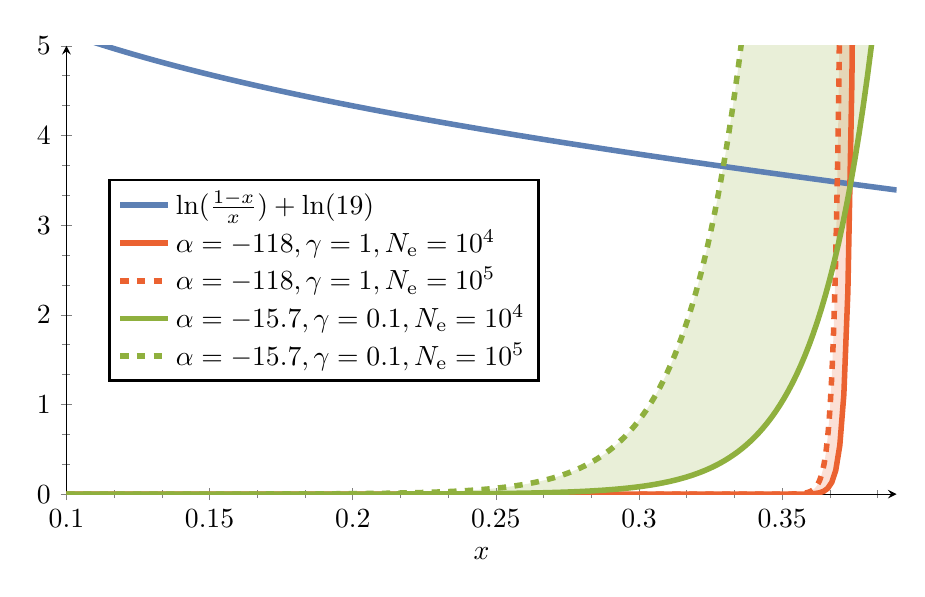
\begin{tikzpicture}
		\begin{axis}[
		width=\textwidth,
		height=\axisdefaultheight,
		xlabel={$\x$},
		ymin=0.0, ymax=5.0,
		samples=200,
		legend entries={$\ln(\frac{1 - \x}{\x}) + \ln(19)$,
			${\alpha = -118, \gamma = 1,\Ne = 10^{4}}$,
			${\alpha = -118, \gamma = 1,\Ne = 10^{5}}$,
			${\alpha = -15.7, \gamma = 0.1,\Ne = 10^{4}}$,
			$\tiny{\alpha = -15.7, \gamma = 0.1,\Ne = 10^{5}}$,
		},
		legend cell align=left,
		minor tick num=2,
		axis x line=bottom,
		axis y line=left,
		legend style={at={(0.05,0.25)},anchor=south west}
		]
		\addplot[domain=0.1:0.39,line width=2.0pt, color=BLUE]{ ln(19*(1-x)/x) };
		\addplot[name path=A, domain=0.1:0.38, line width=2.0pt, color=RED]{4*10000*1.686*exp(1.686*(-118+300*x))};
		\addplot[name path=B, dashed,domain=0.3:0.37, line width=2.0pt, color=RED]{4*100000*1.686*exp(1.686*(-118+300*x))};
		\addplot[name path=C,domain=0.1:0.39, line width=2.0pt, color=GREEN]{4*10000*0.1*1.686*exp(1.686*(-15.71+30*x))};
		\addplot[name path=D,dashed,domain=0.1:0.35, line width=2.0pt, color=GREEN]{4*100000*0.1*1.686*exp(1.686*(-15.71+30*x))};
		\addplot[fill=RED, opacity=0.2] fill between[ of = A and B];
		\addplot[fill=GREEN, opacity=0.2] fill between[ of = C and D];
		\end{axis}
	\end{tikzpicture}
\end{frame}

\begin{frame}
\centering
	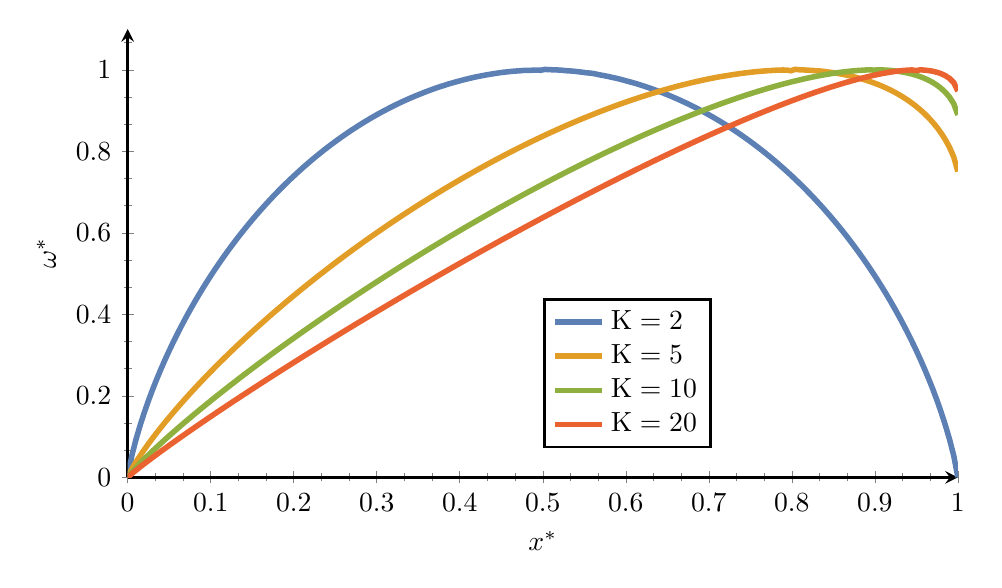
\begin{tikzpicture}[
	declare function={
		omega(\x,\k)= \x*(2*(\x-1)*(ln(\k-1)+ln((1-\x)/\x))/(\k*(\x-1)+1)+ (\k-2)/(\k-1));
	},]
	\begin{axis}[
	width=\textwidth,
	height=\axisdefaultheight,
	ylabel={$\dnds\eq$},
	xlabel={$\x\eq$},
	domain=0:1.0,
	ymin=0.0, ymax=1.1,
	samples=200,
	legend entries={$\Nstate=2$, $\Nstate=5$, $\Nstate=10$, $\Nstate=20$},
	legend cell align=left,
	minor tick num=2,
	axis x line=bottom,
	axis y line=left,
	legend style={at={(0.5,0.4)},anchor=north west}
	]
	\addplot[line width=2.0pt, color=BLUE]{omega(x, 2)};
	\addplot[line width=2.0pt, color=YELLOW]{omega(x, 5)};
	\addplot[line width=2.0pt, color=GREEN]{omega(x, 10)};
	\addplot[line width=2.0pt, color=RED]{omega(x, 20)};
	\end{axis}
	\end{tikzpicture}
\end{frame}

\begin{frame}
\centering
	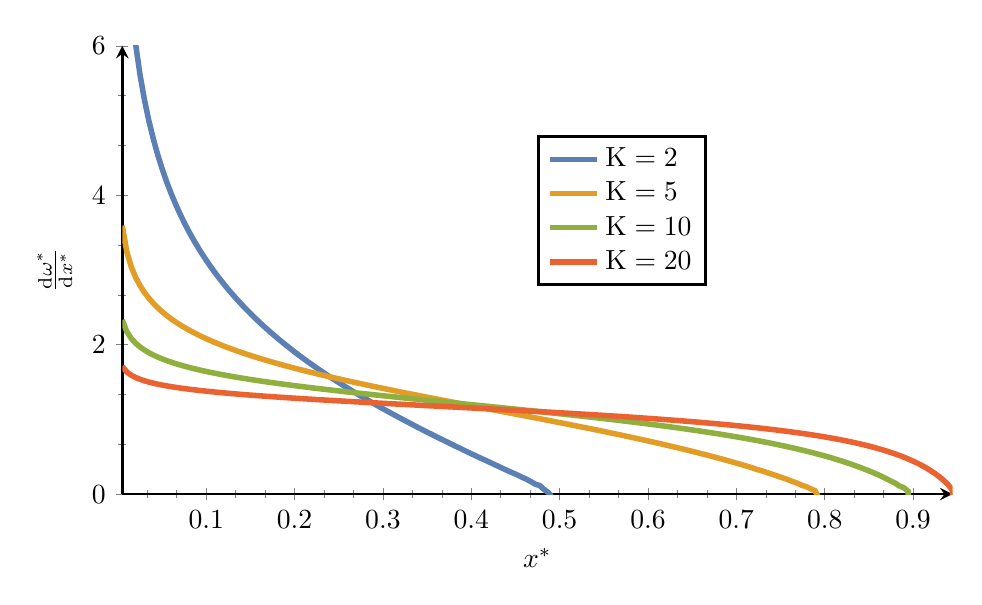
\begin{tikzpicture}[
	declare function={
		domega(\x,\k)= 2*(\k*(\x-1)+1 + (\k*(\x-1)^2+2*\x-1)*(ln(\k-1) + ln((1-\x)/\x)))/(\k*(\x - 1) + 1)^2 + (\k-2) / (\k-1);
	},]
	\begin{axis}[
	width=\textwidth,
	height=\axisdefaultheight,
	ylabel={$\frac{\der \dnds\eq}{\der \x\eq}$},
	xlabel={$\x\eq$},
	domain=0.0:1.0,
	ymin=0, ymax=6,
	samples=200,
	legend entries={$\Nstate=2$, $\Nstate=5$, $\Nstate=10$, $\Nstate=20$},
	legend cell align=left,
	minor tick num=2,
	axis x line=bottom,
	axis y line=left,
	legend style={at={(0.5,0.8)},anchor=north west}
	]
	\addplot[line width=2.0pt, color=BLUE]{domega(x, 2)};
	\addplot[line width=2.0pt, color=YELLOW]{domega(x, 5)};
	\addplot[line width=2.0pt, color=GREEN]{domega(x, 10)};
	\addplot[line width=2.0pt, color=RED]{domega(x, 20)};
	\end{axis}
	\end{tikzpicture}
\end{frame}

\begin{frame}
\centering
	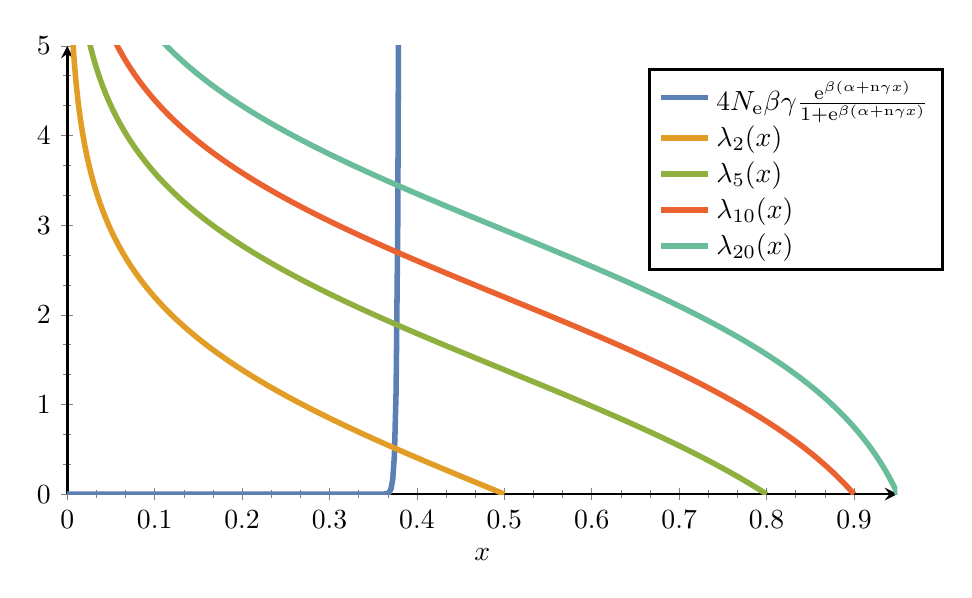
\begin{tikzpicture}[
	declare function={
		lambda(\x,\k)= ln(\k-1) + ln((1-\x)/\x);
	}]
	\begin{axis}[
	width=\textwidth,
	height=\axisdefaultheight,
	xlabel={$\x$},
	ymin=0.0, ymax=5.0,
	samples=200,
	legend entries={
		$4\Ne \beta \gamma \frac{\e^{\beta(\alpha + \Nsite \gamma \x)}}{1 + \e^{\beta(\alpha + \Nsite \gamma \x)}}$,
		$\lambda_{2}(\x)$,
		$\lambda_{5}(\x)$,
		$\lambda_{10}(\x)$,
		$\lambda_{20}(\x)$},
	legend cell align=left,
	minor tick num=2,
	axis x line=bottom,
	axis y line=left,
	legend style={at={(0.7,0.95)},anchor=north west}
	]
	\addplot[domain=0.0:0.38, line width=2.0pt, color=BLUE]{ 4 * 1000 * 1.686 *exp(1.686 * (-118 + 300 *x))};
	\addplot[domain=0.0:0.5,line width=2.0pt, color=YELLOW]{ lambda(x,2) };
	\addplot[domain=0.0:0.8,line width=2.0pt, color=GREEN]{ lambda(x,5) };
	\addplot[domain=0.0:0.9,line width=2.0pt, color=RED]{ lambda(x,10) };
	\addplot[domain=0.0:1.0,line width=2.0pt, color=LIGHTGREEN]{ lambda(x,20) };
	\end{axis}
	\end{tikzpicture}
\end{frame}

\begin{frame}
\begin{figure}[H]
	\centering
	\begin{tikzpicture}[scale = 1.0]
	\begin{axis}[
	width=\textwidth,
	height=\axisdefaultheight,
	ylabel={Fitness $f(\x)$},
	xlabel={Phenotype $\x$},
	cycle list name=colors,
	domain=0:1,
	samples=200,
	legend cell align=left,
	minor tick num=2,
	axis x line=bottom,
	axis y line=left,
	legend entries={$f(\x) = \frac{1}{1 + \e^{\beta(\alpha + \Nsite \gamma \x)}}$},
	legend style={at={(0.4,0.5)},anchor=south west}
	]
	\addplot[line width=2.0pt, color=BLUE]{ 1 / (1+exp(1.686*(-12 + 30 * x)))};
	\addplot[black]{1.0};
	\end{axis}
	\end{tikzpicture}
\end{figure}
\end{frame}

\end{document}